% *****************************************************************************
%     sections/chapter2.tex
%
% Last edit: 16/03
% *****************************************************************************

\chapter{Bayesian inference of neutron star observables}

\section{From the equation of state to neutron star observables}

% Pulsars were identified to rotating NS which produce pulsed emission.
% EoS microscopic -> one wants to evaluate macroscopic properties of the star,
%   such as its mass or radius.
% hydrostatic equilibrium
% plan

\subsection{Masses and radii} 

% observations
From the observational point of view, it is easier for astronomers to measure 
the mass of a NS entering into a binary system. There are several types of
binaries: X-ray binaries, double NS binaries, radio pulsar--white dwarf 
binaries, and radio pulsar--nondegenerate star binaries. Depending on the type 
of binary, different techniques are used to infer the NS 
mass~\cite{Haensel2007}.
% Shapiro delay effect - MSP
For example, in a pulsar binary system, various phenomena, such as the 
relativistic Shapiro delay~\cite{Shapiro1964}, can be measured via pulsar 
timing, which consists of the regular monitoring of the rotation of a a pulsar 
over long periods (years to decades). The relativistic Shapiro delay is a 
phenomenon from which precise masses for both a millisecond pulsar and its 
companion can be inferred~\cite{Demorest2010,Cromartie2020}. Let us notice 
however that it is only observed in a small subset of high-precision, highly 
inclined binary pulsar systems.\\
% Measuring NS radii is less straightforward
Measuring NS radii with high precision is a more challenging task, and it
constitutes one of the goals of the ambitious NICER mission~\cite{NICER}. This
observable can be extracted from the analysis of thermal emission from neutron 
star surfaces, or X-ray emission from accreting neutron stars in binaries.

In the following, we turn to the theoretical prediction of NS masses and radii. 
The hydrostatic equilibrium equations in general relativity are first solved in 
order to represent the mass-radius relation for several popular EoS, which are
then confronted to NS mass measurements. The estimation of the crustal 
thickness and mass is discussed afterwards.

\subsubsection{Mass-radius relation}

% hydrostatic equilibrium in GR
Theoretically, the NS masses and radii correspond to the 
solution of the hydrostatic equilibrium equations, which are, in general 
relativity for spherical and nonrotating stars~\cite{Tolman1939,Oppenheimer1939},
%
\begin{eqnarray}
  \frac{dP}{dr} &=& -\frac{G\rho_B m}{r^2}\left(1 + \frac{P}{\rho_B
  c^2}\right)\left(1+\frac{4\pi
  Pr^3}{mc^2}\right)\left(1-\frac{2Gm}{rc^2}\right)^{-1},\label{eq:tov}\\
      \frac{dm}{dr} &=& 4\pi r^2\rho_B,\label{eq:massbal}\\
  \frac{d\Phi}{dr} &=& -\frac{1}{\rho_B
    c^2}\frac{dP}{dr}\left(1+\frac{P}{\rho_B
  c^2}\right)^{-1}\label{eq:metric},
\end{eqnarray}
%
where $G$ is the gravitational constant, $P$ the pressure, $\rho_B c^2$ the
energy density, and $m(r)$ the is the gravitational mass inside the sphere of
radius $r$, defined within the Schwarzschild metric $ds^2 = c^2dt^2e^{2\Phi} 
- e^{2\lambda}dr^2 - r^2(d\theta^2 + \sin^2\theta d\phi^2)$. The function 
$\Phi(r)$ corresponds to the gravitational potential, and $\lambda(r)$ is 
related to the enclosed mass $m(r)$ through
%
\begin{equation}
  e^{-\lambda} = \sqrt{1-\frac{2Gm}{rc^2}}.
\end{equation}
%
% description of the equations
Eq.~(\ref{eq:tov}) is the so called Tolman-Oppenheimer-Volkoff (TOV) equation 
of hydrostatic equilibrium. The integration of Eq.~(\ref{eq:massbal}) from
$r=0$ to the boundary $r=R$, $R$ being the NS radius, gives the total
gravitational mass $M=m(R)$ of the star. Eq.~(\ref{eq:metric}) is a 
relativistic equation for the metric function $\Phi(r)$. Here, we focus on 
solving Eqs.~(\ref{eq:tov}) and 
(\ref{eq:massbal}), which gives the profiles $P(r)$, $\rho_B(r)$, and $m(r)$ 
for a given EoS, $P(\rho_B)$, the determination of which was discussed in detail 
in Chapter 1.

% explain numerical method for a central density nc (CGS, Euler method, lagrangian interpolation)
In view of solving the hydrostratic equilibrium equations for a given tabulated 
EoS, one first have to choose an arbitrary value for the central density $\rho_{B,c}$ and 
interpolate the central pressure $P_c = P(\rho_{B,c})$, corresponding to $r=0$, 
with the associated boundary condition $m(r=0) = 0$. Then, using a Runge-Kutta 
method, one integrate up to $r=R$, defined as $P(r=R) = 0$ (our numerical 
condition is $P < 5\times 10^{-4}$ MeV/fm$^{3}$, which is a sufficiently low 
value of the pressure). At each new step of pressure, one has to interpolate 
the mass density $\rho_B$ in the table. In the end, for a given value of central 
density $\rho_{B,c}$, one obtains the profiles $P(r)$, $\rho_B(r)$, and $m(r)$, 
and therefore a value for the NS mass $M$ and radius $R$. The typical values 
of these observables are $M=1.4M_\odot$ and $R=10$ km~\cite{Haensel2007}.\\
% The problem is that the central density inside a NS is not known... thats why 
%   we are interested in the Mass radius relation
In fact, the central density inside a specific NS is not known, and is expected
to range from $\approx 4.6\times 10^{14}$ g/cm$^3$ to $\approx 4\times 10^{15}$
g/cm$^3$. For this reason, we are rather interested in the mass-radius relation, which
can be obtained by calculating $M$ and $R$, following the numerical method
previously explained, for this range of central mass densities.\\
% efld
Let us recall that one has to redefine the high-order parameters $Q_{sat(sym)}$ 
and $Z_{sat(sym)}$ in order to reproduce existing functionals at densities
greater than $2n_{sat}$ with the metamodeling technique. This corresponds to
the ELFd technique introduced in \cite{Margueron2018a}.

\begin{table}[!t]
\begin{center}
\begin{tabular}{cccccc} 
  \toprule
  \toprule
  Parameter & Unit & $N$ & BSk14 & PKDD & TM1\\
  \midrule
  $E_{sat}$ & MeV & 0         & -15.85 & -16.27  & -16.26 \\
  $n_{sat}$ & fm$^{-3}$ & 1   & 0.1586 &  0.1495 & 0.1450 \\ 
  $K_{sat}$ & MeV & 2         & 239    &  261    & 281    \\ 
  $Q_{sat}$ & MeV & 3         & -359   &  -119   & -285   \\ 
  $Z_{sat}$ & MeV & 4         & 1435   &  4213   & 2014   \\ 
  $E_{sym}$ & MeV & 0         & 30.00  &  31.19  & 36.94  \\
  $L_{sym}$ & MeV & 1         & 43.9   &  79.5   & 111.0  \\
  $K_{sym}$ & MeV & 2         & -152   &  -50    & 34     \\
  $Q_{sym}$ & MeV & 3         & 389    &  -28    & -67    \\
  $Z_{sym}$ & MeV & 4         & -2191  &  -1315  & -1546  \\
  $m_{sat}^*/m$ & &           & 0.80   &  0.65   & 0.71   \\
  $\Delta m_{sat}^*/m$ & &    & 0.03   &  -0.08  & -0.09  \\
  \bottomrule
  \bottomrule
\end{tabular}
\end{center}
\caption[Empirical parameters for BSk14, PKDD, and TM1]{Empirical parameter and 
  associated unit and derivative order $N$ for BSk14 \cite{Goriely2007}, PKDD
  \cite{Long2004}, and TM1~\cite{Sumiyoshi1995} functionals.}\label{table:newemppar}
\end{table}

\begin{figure}[!t]
\begin{center}
  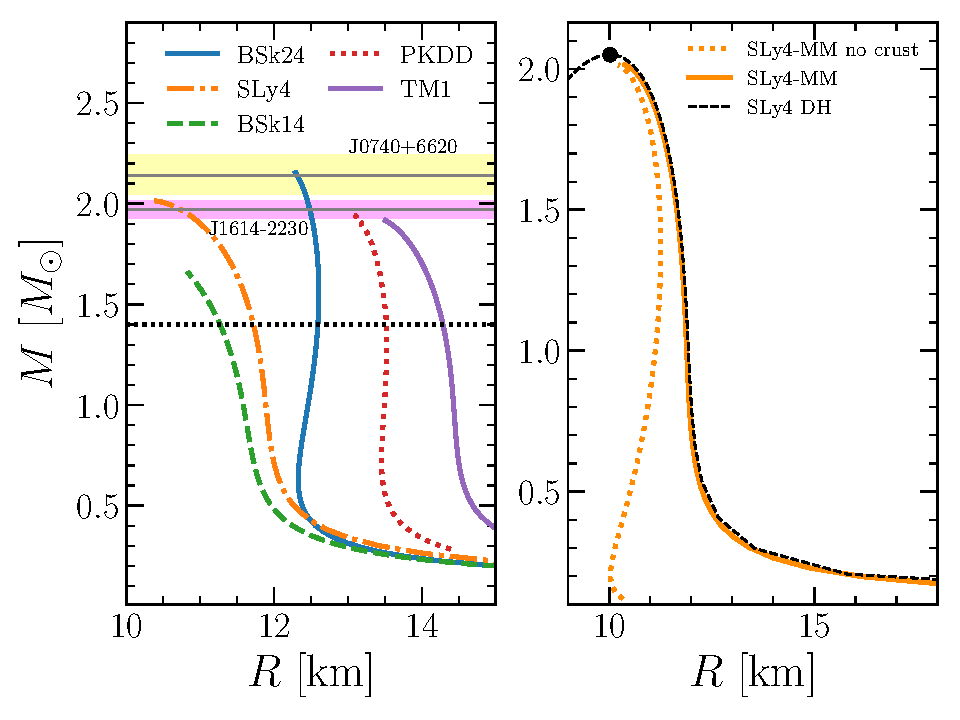
\includegraphics[width=0.9\linewidth]{figures/mr_popular.pdf}
\end{center}
\caption[Mass-radius relation for several popular EoS]{Left: Mass-radius 
  relation for several popular EoS calculated
  with the metamodeling technique. The black dotted line marks the NS 
canonical mass, that is $1.4M_\odot$. The magenta band represents the measured 
mass of J1614-2230, $(1.97 \pm 0.04)M_\odot$ \cite{Demorest2010}, and the 
yellow band that of J0740+6620, $2.14_{-0.09}^{+0.10}M_\odot$ ($68.3\%$ 
credibility interval) \cite{Cromartie2020}.
Right: Mass-radius relation for the DH EoS for SLy4 functional (black dashed
line), and the SLy4 EoS calculated with the metamodeling technique (solid
orange line). The black circle indicates the maximum mass.}\label{fig:mr_popular}
\end{figure}
 
The left panel of Fig.~\ref{fig:mr_popular} shows the mass-radius relation for 
several popular EoS based on Skyrme-type functionals BSk24, SLy4, and BSk14, 
and relativistic models PKDD and TM1, calculated within the metamodeling 
technique. A strong model dependence is observed, with radii of canonical NS 
ranging from $R_{1.4}=11.5$ km for BSk14 to $R_{1.4}=14.5$ km for TM1. More
specifically, it is seen that the radius is positively correlated to the slope 
of the symmetry energy $L_{sym}$. The value of the empirical parameters 
associated to BSk14, TM1, and PKDD are reported in Table~\ref{table:newemppar}, 
whereas those of BSk24 and SLy4 can be found in Table~\ref{table:emp_params}.\\
The bands correspond to the measured masses of the two most massive
pulsars observed to the present day. The mass of J1614-2230 was precisely 
estimated to $(1.97\pm 0.04)M_\odot$~\cite{Demorest2010}, and the very recent
relativistic Shapiro delay measurements of J0740+6620 led to 
$2.14_{-0.09}^{0.10}M_\odot$ ($68.3\%$ credibility
interval)~\cite{Cromartie2020}. Naturally, if an
EoS cannot insure such high masses, it should not be considered as reliable, 
in particular at high density, since the maximum mass is determined by the 
stellar core EoS. In particular, it is seen that the maximum mass corresponding
to the BSk14 functional, $1.8M_\odot$, is lower than the measured mass
of J1614-2230. Also, while the SLy4 EoS satisty this constraint, the maximum 
mass for this EoS, $2.05M_\odot$, is lower than that of J0740+6620. This 
outline the fact that measuring the mass of pulsars is important, because it 
provides a strong constraint on the stellar matter EoS. Similarly, the NICER
telescope is expected to provide, for years to come, a constraint on the NS
radii with a precision of $5\%$. Ultimately, in the ideal case where one could 
accurately measure the mass and radius of one neutron star, it would be possible 
to determine the EoS by positioning the point in the $M-R$ diagram.

The mass-radius relation for the SLy4 EoS is represented in the right panel of
Fig.~\ref{fig:mr_popular}. The solid orange line corresponds to $M(R)$ for the 
SLy4 EoS calculated within the metamodeling technique, and the dashed 
black line is the calculation based on the DH EoS for SLy4 functional. A perfect
agreement is observed between the two curves, reflecting the small error on the
EoS, illustrated in Fig.~\ref{fig:unified}. \\
The dotted orange line shows the mass-radius relation for the SLy4 EoS without
considering the clustering of matter at low density, that is assuming that the
NS star interior consists of $npe\mu$ matter at all densities. In that case,
for a canonical NS, we find $R_{1.4} = 11.1$ km, which is almost $1$ km lower 
with respect to the result with a crust EoS. Moreover, this difference is found 
to be larger with decreasing mass. This shows that the crust EoS is essential 
to properly predict NS radii. However, we can see that the NS maximum mass is 
entirely determined by the stellar core EoS.\\
The black point marks the maximum mass for the SLy4 EoS, $M_{max} = 2.05M_\odot$. 
Let us notice that the branch left to the point is unstable, 
because from this point the mass decreases with central density increasing.

\subsubsection{Crust thickness and mass}
% crust thickness and mass
As explained in Chapter 1, a precise estimation of the CC transition point is
required as far as crustal properties are concerned. In particular, the
transition pressure $P_t$ is essential for the determination of the thickness 
and mass of the crust, given respectively by $l_{crust}=R-R_{core}$ and
$M_{crust}=M-M_{core}$, with $R_{core}$ ($M_{core}$) the radius
(mass) of the stellar core. Indeed, in order to caclulate the core radius and
mass, which are involved in the calculation of the crustal observables, one has 
to integrate the hydrostatic equilibrium equations, Eqs.~(\ref{eq:tov}) and 
(\ref{eq:massbal}), from $r=0$ to $r=R_{core}$, defined as $P(r=R_{core})=P_t$.

\begin{figure}[!t]
\begin{center}
  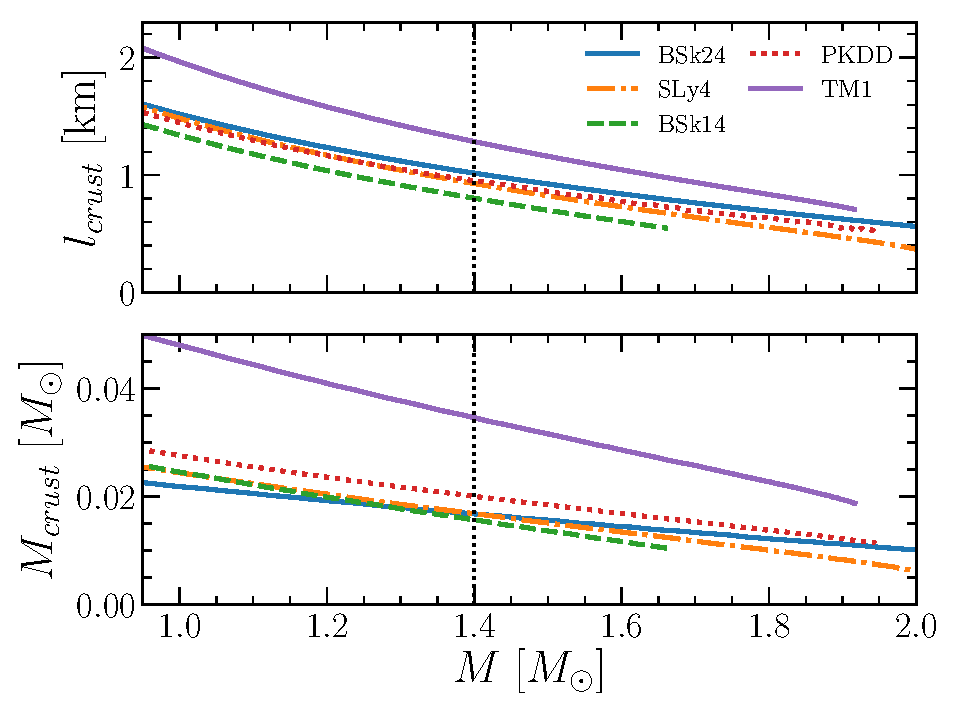
\includegraphics[width=0.9\linewidth]{figures/crustmassthick.pdf}
\end{center}
\caption[Crust thickness and mass versus NS mass for several popular EoS]{Crust 
  thickness $l_{crust}$ (upper panel) and mass $M_{crust}$ (lower panel) as a function of 
  the NS mass $M$ for several popular EoS calculated within the metamodeling
technique. The black dotted line marks the NS canonical mass, that is 
$1.4M_\odot$.}\label{fig:crustmassthick}
\end{figure}

Fig.~\ref{fig:crustmassthick} shows the variation with NS mass of crust 
thickness $l_{crust}$ and mass $M_{crust}$ for the same EoS as in 
Fig.~\ref{fig:mr_popular}. As previously, the high-order empirical parameters
are reevaluated to calculate the EoS entering into the TOV equation. However,
the transition pressure is calculated using the values of $Q_{sat(sym)}$ and
$Z_{sat(sym)}$ directly derived from the selected functionals. The reason is
that, as showed in Fig.~\ref{fig:sly4_nt}, the determination of CC transition 
point is sensitive to orders $N>2$.\\
We find the interesting result that the crust is thicker for low-mass neutron 
stars, and in consequence that the $M_{crust}$ drops continuously with 
increasing NS mass. At $M=1.4M_\odot$ (black dotted line), we 
observe that the crust is $\approx 1$ km thick, and that the crust mass is 
approximately $0.02-0.04M_\odot$, which is $(1.5-3)\%$ of the total mass. Once
again, a model dependence is observed. Nonetheless, the correlation of the 
crust thickness with the slope of the symmetry energy is 
not clear. In Fig.~\ref{fig:mr_popular}, we have seen that the radius of the 
star is positively correlated with $L_{sym}$. In fact, the same is true for the 
core radius, explaining why the correlations cancel in the crust 
thickness $l_{crust} = R - R_{core}$.

\subsection{Moment of inertia within the slow rotation approximation}

We now turn to the calculation of the moment of inertia within the slow rotation 
approximation~\cite{Hartle1967}. In 
fact, this approximation is not only applicable to slowly rotating pulsars but 
is also reliable for most of them. Indeed, while many observed pulsars show  
rapid rotation~\cite{Stovall2013}, their structure is almost not altered by it 
since centrifugal forces are small in comparison to the gravity, 
$R^3\Omega^2/(GM) \ll 1$, $\Omega$ being the angular frequency. For instance, 
let us consider a rapidly rotating pulsar with $\Omega = 1000$ s$^{-1}$ and 
canonical values for its mass and radius, $M=1.4M_\odot$ and $R=10$ km. In that 
case, we find $R^3\Omega^2/(GM) \approx 0.025$.

In the following, we first calculate the total moment of inertia and the 
fraction of it contained in the NS crust for several popular EoS. Then, we 
explain the connection between the fraction of crust moment of inertia 
and the glitch behavior exhibited by some pulsars~\cite{Espinoza2011}.

\subsubsection{Total moment of inertia and fraction contained in the crust}

In a slowly rotating NS, the total moment of inertia is given
by~\cite{Hartle1967}
%
\begin{equation}
  I = \frac{8\pi}{3}\int_0^R dr r^4\left(\rho_B +
  \frac{P}{c^2}\right)\frac{\bar{\omega}}{\Omega}e^{-\lambda-\Phi}\label{eq:moi},
\end{equation}
%
where we have introduced the rotational drag function $\bar{\omega}(r)$, which
satisfies
%
\begin{equation}
  \frac{d}{dr}\left(r^4j\frac{d\bar{\omega}}{dr}\right) =
  -4r^3\bar{\omega}\frac{dj}{dr},\label{eq:rotdrag}
\end{equation}
%
with $j=e^{-\Phi-\lambda}$. Eq.~(\ref{eq:rotdrag}) satisfy the following
boundary conditions at the surface and center of the NS, respectively:
%
\begin{equation}
  \frac{1}{\Omega}\bar{\omega}(r=R) = 1 - \frac{2GI}{R^3c^2} \quad \text{and} 
  \quad \frac{d\bar{\omega}}{dr}\bigg|_{r=0} = 0.
\end{equation}
%
One can translate Eq.~(\ref{eq:rotdrag}) into a first-order differential
equation by introducting $w = (1/\Omega)d\ln\bar{\omega}/d\ln r$, yielding
%
\begin{equation}
  \frac{dw}{dr} = \frac{4\pi G}{c^2}\frac{(P+\rho_Bc^2)(4+w)r^2}{rc^2-2Gm} -
  \frac{w}{r}(3+w)\label{eq:rotdrag2},
\end{equation}
%
with the boundary condition $w(r=0) = 0$. This equation is solved together with 
Eqs.~(\ref{eq:tov}) and (\ref{eq:massbal}) in order to calculate the total 
moment of inertia, which can be rewritten as
%
\begin{equation}
  I = \frac{c^2}{G}\frac{w(R)R^3}{6 + 2w(R)}.
\end{equation}
%
The fraction of crust moment of inertia can also be calculated as~\cite{Lim2019}
%
\begin{eqnarray}
  \frac{I_{crust}}{I} &=& 1 - \frac{I_{core}}{I}\notag\\
                      &=& 1 - \left(\frac{R_{core}}{R}\right)^3
                      \frac{w(R_{core})}{w(R)}
                      \exp\left[-\int_{R_{core}}^{R}\frac{w(r)}{r}dr\right],
\end{eqnarray}
%
where we have introduced the moment of inertia of the core $I_{core}$, defined
by the integration of Eq.~(\ref{eq:moi}) up to the core radius $R=R_{core}$.

\begin{figure}[!t]
\begin{center}
  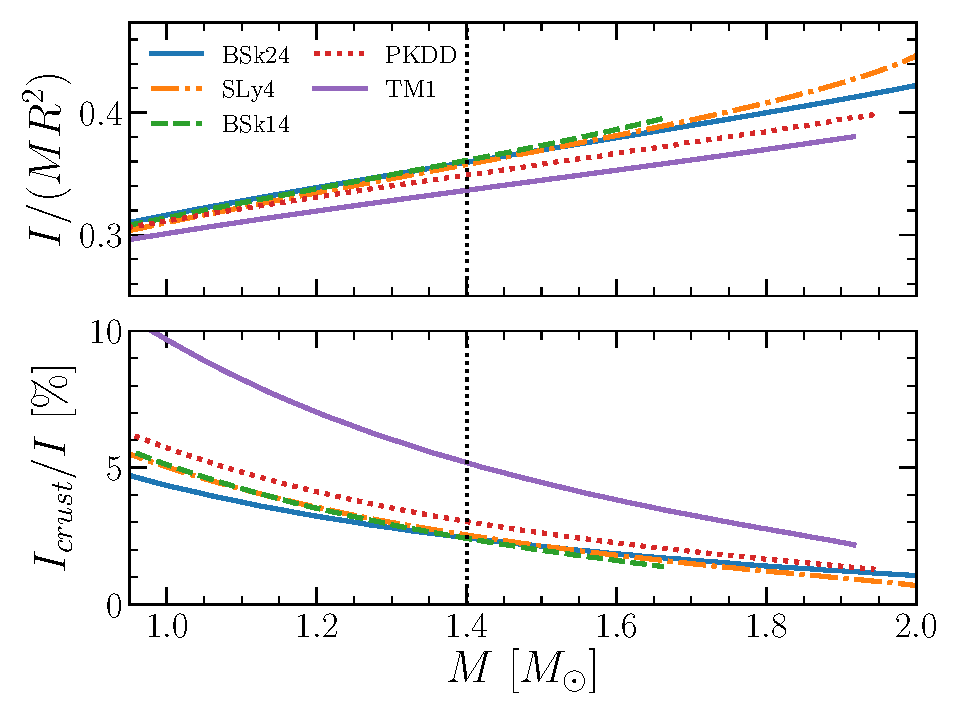
\includegraphics[width=0.9\linewidth]{figures/moi_popular.pdf}
\end{center}
\caption[Moment of inertia and fraction of crust moment of inertia
versus NS mass for several popular EoS]{Moment of
  inertia $I$ (upper panel) and fraction of crust moment of inertia
  $I_{crust}/I$ (lower panel) as a function of the NS mass $M$ for several 
  popular EoS calculated within the metamodeling technique. In the upper panel, 
  the black dotted line marks the NS canonical mass, that is $1.4M_\odot$. In
the lower panel, the minimum values needed to justify Vela glitches with
(Delsate \textit{et al.}~\cite{Delsate2016} and Andersson \textit{et
al.}~\cite{Andersson2012}) and without (Link \textit{et al.}~\cite{Link1999}) 
crustal entrainment are represented.}\label{fig:moi_popular}
\end{figure}

The total moment of inertia is plotted as a function of the NS mass in the
upper panel of Fig.~\ref{fig:moi_popular} for EoS based on Skyrme-type
functionals BSk24, SLy4, and BSk14, and relativistic models PKDD and TM1.
For $M=1.4M_\odot$, it is found that $I$ ranges from $\approx 1.2\times 10^{45}$
g cm$^2$ for the soft BSk14 EoS to $\approx 2\times 10^{45}$ g cm$^2$ for the 
very stiff TM1 EoS. This shows the strong dependence on the EoS. More 
particularly, an apparent positive correlation with $L_{sym}$ is observed. 
It is seen that the model dependence is even larger for high-mass NS.

The lower panel of Fig.~\ref{fig:moi_popular} shows the variation with NS mass
of $I_{crust}/I$ for the same EoS. It is seen that the more massive a 
NS is, the less moment of inertia it stores in its crust, which follows
the trends observed in Fig.~\ref{fig:crustmassthick}. This was predictable from 
the sensitivity of crustal properties to the CC transition pressure. Given the 
selected EoS, the value of $I_{crust}/I$ at $M=1.4M_\odot$ 
ranges from $\approx 2\%$ for BSk14 to $\approx 5\%$ for TM1, showing once 
again the dramatic dependence on the EoS.

\subsubsection{Connection to pulsar glitches}

The so-called pulsar glitches, which are sudden jumps in the rotational 
frequency of a compact star, are thought to originate from an abrupt 
transfer of angular momentum from the neutron superfluid to the solid crust of 
the star due to the unpinning of the superfluid vortices from the crystal
lattice~\cite{Anderson1975}. %elaborate a bit more: why do vortices unpin?

At the time of writing, 555 glitches have been observed in 190 pulsars through 
high-precision pulsar timing~\cite{Espinoza2011,Glitches}. For a given 
glitcher, three quantities are usually measured: its spin frequency $\Omega$, 
its average spin-down rate $\dot{\Omega}$, and its glitch activity parameter
$\mathcal{A}$, defined as
%
\begin{equation}
  \mathcal{A} = \frac{1}{t}\sum_{i=1}^{N} \frac{\Delta \Omega_i}{\Omega},
\end{equation}
%
where $\sum_i \Delta\Omega_i/\Omega$ represents the cumulative spin-up rate
over the $N$ glitches occuring during a time $t$.

It was demonstrated in~\cite{Link1999} that the ratio of the moment of inertia
associated to the neutron superfluid which drives the glitches $I_{sf}$ to the 
moment of inertia of the solid crust -- plus any portion of the star strongly 
coupled to it -- $I_c$ must satisfy 
%
\begin{equation}
  \frac{I_{sf}}{I_c} \geq \frac{\Omega}{|\dot{\Omega}|}\mathcal{A} 
  \equiv \mathcal{G},
\end{equation}
%
where we have introduced the coupling parameter $\mathcal{G}$. In view of
relating the observational constraint $\mathcal{G}$ to the fractional moment of
inertia $I_{crust}/I$ to ultimately set a constraint on the stellar EoS, we 
assume that the angular momentum reservoir is confined to the neutron 
superfluid coexisting with the crystal lattice of the inner crust. In that 
case, we have $I_c = I - I_{res} \simeq I$ and $I_{crust} \simeq I_{sf}$,
yielding~\cite{Link1999}
%
\begin{equation}
  \frac{I_{sf}}{I_c} \simeq \frac{I_{crust}}{I} \geq \mathcal{G}\label{eq:noent}.
\end{equation}
%

% blabla entrainment (origin, ratio mn*/mn can be high)
Taking into account the entrainment coupling, the previous constraint, 
Eq.~(\ref{eq:noent}), becomes~\cite{Andersson2012}
%
\begin{equation}
  \frac{I_{crust}}{I} \geq \mathcal{G}\frac{\langle m_n^* \rangle}{m_n},
\end{equation}
%
with $\langle m_n^* \rangle$ the average effective neutron mass.
It should be stressed that systematic calculations of $m_n^*$ throughout 
the NS crust are very costly from the computational point of view and that,
following~\cite{Andersson2012,Piekarewicz2014}, we adopt the value $\langle m_n^* \rangle 
/m_n = 4.3$, which is inferred from the results of~\cite{Chamel2012}. 
Naturally, one recover the expression without crustal entrainment in the case 
of $\langle m_n^* \rangle = m_n$.

The Vela pulsar (B083345-45) is one of the most active glitchers known, with
glitches occuring four times per decade on average. Since the beginning of its 
monitoring, almost than 50 years ago, it has exhibited 20 glitches in
total~\cite{Glitches}, allowing for a precise estimation of the corresponding 
the coupling parameter, $\mathcal{G}_{Vela} = (1.62 \pm 0.03) \times
10^{-2}$~\cite{Ho2015}. This can be translated into a constraint for 
the fraction of crust moment of inertia,
%
\begin{equation}
  \left(\frac{I_{crust}}{I}\right)_{Vela} \geq (1.62 \pm 0.03) \times 10^{-2}
  \frac{\langle m_n^* \rangle}{m_n} \approx 0.07.
\end{equation}
%
In other words, in the hypothesis that the angular momentum reservoir is 
exclusively confined to the neutron superfluid permeating the inner crust, the 
crust must store more than $7\%$ of the total moment of inertia in order to 
justify the large glitches occuring in the Vela pulsar.\\
% discuss the 'is the crust enough?' problem with Fig. 3
We show in Fig.~\ref{fig:moi_popular} blabla.
Finally, due to model dependence, is not clear whether the superfluid 
neutron in the crust can carry enough angular momentum to explain Vela 
glitches. For this reason, the question will be addressed 
in~\ref{subsec:gli_stats} in the context of a complete statistical analysis.

\subsection{Tidal deformability} % 2

% observable of interest since gw170817 event
% explain tidal deformability (dimless, lambda1-lambda2, lambda tilde...)
% derive equations from k2 love number
% figure
% discussion

\section{Bayesian modeling of the equation of state} % 0.75

% explain motivation (more and more observations with technical progress,
%   observations and nuclear physics are complementary)

\subsection{Principle of Bayesian inference} % 1.5

% expressions
% discussions

\subsection{Prior distribution from nuclear experiments} % 2

\subsection{Sensitivity analysis} % 3
% ... on the crust-core transition point?

\subsection{Filters} % 0.25

\subsubsection{Low-density filters from ab initio calculations} % 2.5

% discuss ab initio calculations (saturation properties, max is 0.2, etc.)
% should we consider the pressure as a filter or not? (bsk24 does not fit in
%   the band)
% +/- 10% to account for other ab initio calculations

\subsubsection{High-density filters from astrophysical observations and 
physical requirements} % 1.5

% symmetry energy positive is a debatable hypothesis (see remark of referee)
% maximum mass as a sharp filter? 1.97? 2.23?
% more constraints in the future with nicer and lvc

\subsection{Posterior distribution of empirical parameters} % 3

% discuss the importance of filters?

\section{General predictions for neutron star observables} % 0.75

% should i add a subsection 'Posterior distribution of NS observables'?

\subsection{Confrontation with GW170817 event} % 1

\subsubsection{Equation of state} % 1

\subsubsection{Mass-radius relation} % 1.5

% speed of sound expansion allows for phase transition, unlike the mm
% -> lower radius found in 1908.10352 could be the sign of a pt to quarks?

\subsubsection{Tidal deformability} % 2

% was measured for the first time for gw170817 event allowing to calculate the
%   m1-m2, lambda1-lambda2 relations

\subsection{Bayesian analysis of the crust-core transition} % 4

% surface figures (prior/posterior)
% corr(Pt,Ksym) (link with chapter 1)
% correlation with isovector bulk parameters is softened if one consider p as a
%   free parameters (see corr matrix)

\subsection{Crustal moment of inertia and pulsar
glitches}\label{subsec:gli_stats} % 4

% explain pulsar glitches phenomena
% give the hypothesis explaining the phenomena
% superfluid neutrons in the crust
% is the crust enough? -> bayesian approach to consider every models (not only
%   relativistic or skyrme functionals as two separate families)
% the crust moment of inertia is calculated following eq given in 2.1.2. the
%   calculation is stopped at the crust-core interface
% report results

\section{Conclusion} % 1

% word on machine learning
